% Main document for Overleaf. Three pdfLaTeX passes settle the contents.
\documentclass[11pt,a4paper]{article}
\usepackage[T1]{fontenc}
\usepackage[utf8]{inputenc}
\usepackage[french]{babel}
\frenchsetup{SmallCapsFigTabCaptions=false}
\usepackage{lmodern}
\usepackage[a4paper,margin=2.15cm,footskip=1cm,headheight=14pt,headsep=0.5cm]{geometry}
\usepackage{amsmath,amssymb}
\usepackage{graphicx,booktabs,float}
\usepackage[font=small,labelfont=bf]{caption}
\usepackage{xcolor}
\definecolor{navy}{HTML}{19334D}
\usepackage{titlesec}
\titleformat{\section}{\large\bfseries\color{navy}}{\thesection}{0.6em}{}
\titleformat{\subsection}{\normalsize\bfseries}{\thesubsection}{0.6em}{}
\titlespacing*{\section}{0pt}{1.1em}{0.45em}
\titlespacing*{\subsection}{0pt}{0.8em}{0.35em}
\usepackage[hidelinks]{hyperref}
\hypersetup{pdftitle={Clustering sous contrainte d'ordre — Programmation dynamique de Fisher},
            pdfsubject={Projet de clustering, Master MLSD, 2026–2027},
            pdfkeywords={segmentation, Fisher, Bellman, K-means, Ward}}
% Authors are listed alphabetically by surname.
\newcommand{\ReportAuthors}{Wael AKIL\\Jinyu CONG\\Furkan NARIN}
\newcommand{\ReportUniversity}{Université Paris Cité}
\newcommand{\ReportFaculty}{UFR des Sciences fondamentales et biomédicales}
\newcommand{\ReportProgramme}{Master 2 Informatique}
\newcommand{\ReportTrack}{Machine Learning pour la Science des Données}
\newcommand{\ReportCourse}{2026/2027}
\newcommand{\ReportShortTitle}{Clustering sous contrainte d'ordre}
\newcommand{\ReportHeaderProgramme}{Master 2 MLSD}
\newcommand{\ReportDate}{22 novembre 2026}

\pdfstringdefDisableCommands{\def\\{, }}
\hypersetup{pdfauthor={\ReportAuthors}}
\newcommand{\PcaOne}{51{,}8}
\newcommand{\PcaTwo}{25{,}1}

\setlength{\parindent}{0pt}
\setlength{\parskip}{0.4em}
\setlength{\textfloatsep}{0.65em}
\setlength{\intextsep}{0.65em}
\setlength{\abovedisplayskip}{0.55em}
\setlength{\belowdisplayskip}{0.55em}
\renewcommand{\arraystretch}{1.12}
\graphicspath{{figures/}}
\newcommand{\R}{\mathbb{R}}
\newcommand{\norm}[1]{\left\lVert#1\right\rVert}
\newcommand{\file}[1]{\texttt{\detokenize{#1}}}
% Fixed running title on body pages; preliminary pages retain plain numbering.
\makeatletter
\def\ps@report{%
  \def\@oddhead{\normalfont\small\color{navy}\ReportShortTitle\hfil\ReportHeaderProgramme}%
  \let\@evenhead\@oddhead
  \def\@oddfoot{\normalfont\hfil\thepage\hfil}%
  \let\@evenfoot\@oddfoot
}
\makeatother
\raggedbottom
\begin{document}
\hypersetup{pageanchor=false}
\begin{titlepage}
\thispagestyle{empty}
\begin{center}
  
\includegraphics[width=5.2cm]{assets/universite-paris-cite-logo.pdf}\par
  \vspace{0.6cm}
  {\large\bfseries\ReportUniversity}\par
  \vspace{0.3em}
  \ReportFaculty\par
  \vspace{1.1cm}
  {\large\ReportProgramme}\par
  \vspace{0.3em}
  \ReportTrack\par
  \vspace{0.4em}
  {\small\ReportCourse}\par
  \vspace{2.4cm}
  {\LARGE\bfseries\color{navy} Clustering sous contrainte d'ordre}\par
  \vspace{0.6em}
  {\Large Programmation dynamique de Fisher}\par
  \vspace{1.8cm}
  \ReportAuthors\par
  \vspace{0.7em}
  \ReportDate
\end{center}
\vfill
\end{titlepage}

\clearpage
\hypersetup{pageanchor=true}
\pagenumbering{roman}
\begingroup
\titleformat{name=\section,numberless}{\centering\large\bfseries\color{navy}}{}{0pt}{}
\section*{Résumé}
Nous étudions la partition d'une séquence en segments contigus par minimisation
exacte de l'inertie intra-classe. La méthode de Fisher est comparée aux K-means
et à la classification ascendante hiérarchique de Ward. Sur les données simulées,
le coude du critère conduit à quatre segments. Sur \file{aiguillage}, Fisher
retrouve les quatre classes de référence, avec un ARI de 1, contre $0{,}943$
pour les K-means à 20 départs et $0{,}859$ pour Ward. Les analyses
complémentaires montrent toutefois que la comparaison dépend de l'initialisation
des K-means et de l'échelle des variables.

\clearpage
\tableofcontents
\clearpage
\renewcommand{\listfigurename}{Liste des figures}
\renewcommand{\listtablename}{Liste des tableaux}
\listoffigures
\clearpage
\listoftables
\endgroup
\clearpage
\pagenumbering{arabic}
\pagestyle{report}
\section{Introduction}
\subsection{Objectif}
Nous étudions l'apport de la contrainte d'ordre pour identifier des régimes
homogènes dans une séquence. Fisher est comparé aux K-means et à la CAH de Ward
sur \file{sequencesimu}, puis sur \file{aiguillage} à quatre classes.
Une classe doit ici former un intervalle : des groupes proches dans l'espace
peuvent correspondre à des régimes temporels différents.

\subsection{Données et démarche}
\begin{table}[H]
\centering\small
\begin{tabular}{lrrl}
\toprule
Fichier & Observations $n$ & Variables $p$ & Référence disponible \\
\midrule
\file{sequencesimu.txt} & 160 & 2 & Aucune étiquette fournie \\
\file{aiguillage.txt} & 140 & 552 & Colonne 553 : quatre classes \\
\bottomrule
\end{tabular}
\caption[Données analysées]{Données analysées. Les lignes restent dans leur ordre d'origine.}
\label{tab:donnees}
\end{table}

La colonne de référence de \file{aiguillage} est séparée des variables avant
tout ajustement. Les 552 coordonnées contribuent au calcul des distances.

La démarche comporte trois étapes : définir et vérifier le critère de Fisher,
choisir le nombre de segments sur les données simulées, puis évaluer les
partitions réelles. Les expériences d'initialisation et de changement d'échelle
évaluent la sensibilité des partitions.

\section{Méthode et protocole expérimental}
\subsection{Critère de segmentation}
Pour $x_i\in\R^p$, le coût d'un segment $[a,b]$ est sa somme des carrés
autour du barycentre, suivant le critère d'homogénéité de Fisher
\cite{fisher} :
\begin{equation}
 \mu_{a:b}=\frac{1}{b-a+1}\sum_{i=a}^{b}x_i,
 \qquad D(a,b)=\sum_{i=a}^{b}\norm{x_i-\mu_{a:b}}^2.
 \label{eq:segment}
\end{equation}
Avec $s_0=1<s_1<\dots<s_{K-1}<s_K=n+1$, la partition est formée des
intervalles $[s_{k-1},s_k-1]$ et minimise
\begin{equation}
 C(s_1,\dots,s_{K-1})=\sum_{k=1}^{K}D(s_{k-1},s_k-1).
 \label{eq:objectif}
\end{equation}
Les segments sont non vides, disjoints et couvrent toutes les observations.
Cette écriture conserve l'inertie du clustering euclidien, mais restreint
l'ensemble des partitions admissibles à celles respectant l'ordre.

\subsection{Programmation dynamique}
Soit $M(i,k)$ le coût minimal des $i$ premières observations en $k$ segments :
\begin{align}
 M(i,1)&=D(1,i),\label{eq:base}\\
 M(i,k)&=\min_{t=k,\dots,i}\bigl\{M(t-1,k-1)+D(t,i)\bigr\},
 \quad 2\leq k\leq K,\ i\geq k.\label{eq:recurrence}
\end{align}
Le tableau $A$ conserve l'argument du minimum ; la reconstruction remonte de
$(n,K)$ à $(t-1,k-1)$, avec $t=A(i,k)$. Le principe d'optimalité garantit
le minimum global à $K$ fixé : chaque préfixe retenu est optimal \cite{fisher}.

Dans \file{fisherDP.py}, \file{diam} calcule \eqref{eq:segment} et
\file{clustfisher} retourne le modèle, les coupures et les labels.
Le critère est stocké dans \file{inertia_}. La récurrence coûte $O(Kn^2)$ ; le calcul
direct de $D$ ajoute $O(n^3p)$, avec une mémoire $O(n^2+nK)$.

\subsection{Comparateurs et prétraitement}
Les \textbf{K-means} alternent affectation et calcul des barycentres, avec un
optimum local dépendant de l'initialisation \cite{lloyd}.
La \textbf{CAH de Ward} fusionne les groupes en augmentant le moins possible
l'inertie ; une coupe fournit $K$ classes \cite{ward}.
Ces méthodes ignorent l'ordre.

Le protocole principal est le suivant : variables brutes en \file{float32},
Ward euclidien et K-means (initialisation \file{k-means++}, \file{n_init=20},
\file{random_state=42}) ; le départ de moindre inertie est retenu \cite{sklearn}.
Les départs multiples limitent le risque de retenir un optimum local défavorable.
L'ACP, calculée par SVD complète après centrage-réduction, sert seulement à
l'affichage des données réelles ; les modèles utilisent
552 variables. La section~\ref{sec:sensibilite} étudie les variantes du protocole.

\subsection{Évaluation et vérification}
L'inertie est recalculée pour chaque partition. L'\textbf{ARI} compare les paires
d'individus, en corrigeant l'accord attendu par hasard ; il vaut 1 pour des
partitions identiques à permutation près \cite{hubert}. Le \textbf{taux de bonne classification}
est \cite{same}
\begin{equation}
 \mathrm{TBC}=\frac{1}{n}\max_{\pi}\sum_{i=1}^{n}
 \mathbf{1}\{y_i=\pi(\widehat z_i)\}.
 \label{eq:tbc}
\end{equation}
L'algorithme hongrois aligne les labels pour le TBC et les matrices de confusion ;
l'ARI ne nécessite aucun alignement. Les changements entre labels voisins
mesurent la fragmentation, pas l'exactitude.

Les entrées vides, non finies et les valeurs illégales de $K$ sont rejetées.
Les coûts et les coupures de Fisher sont vérifiés indépendamment par
énumération exhaustive sur 270 cas :
$n=1,\dots,9$, $p\in\{1,2,4\}$, tous les $K$ légaux,
\file{float32}/\file{float64}, tolérances relative $2\times10^{-6}$ et absolue $10^{-6}$.

\section{Application aux données simulées}
\subsection{Choix de K et coupures}
Le coude du critère $C$ de Fisher conduit à $K=4$ (figure~\ref{fig:coude})
\cite{same}. Les valeurs à $K=3,4,5$ sont
$462{,}01$, $300{,}60$, $292{,}37$ : le gain passe de $161{,}42$ à $8{,}22$
(de $34{,}9\,\%$ à $2{,}7\,\%$).
Minimiser directement $C$ sur $K$ serait inadapté, car $K=n$ donne zéro.

\begin{figure}[H]
\centering
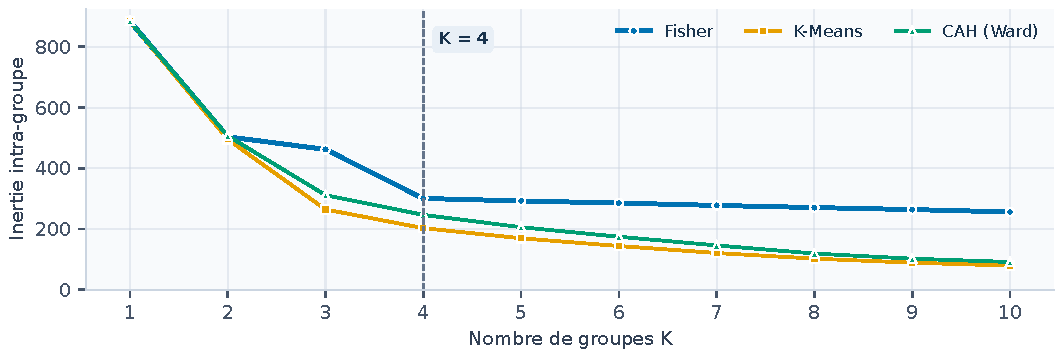
\includegraphics[width=0.94\linewidth,height=4.7cm,keepaspectratio]{simulation_coude.pdf}
\caption[Simulation : inertie et choix du nombre de segments]{Inerties sur \file{sequencesimu}. Le trait vertical indique $K=4$ ;
les K-means utilisent 20 départs, graine 42.}
\label{fig:coude}
\end{figure}
Les coupures Python sont $[50,80,130]$, soit $[51,81,131]$ en numérotation à partir de 1.
Les segments $1$--$50$, $51$--$80$, $81$--$130$, $131$--$160$ ont pour
effectifs $[50,30,50,30]$.

\subsection{Comparaison des partitions}
\begin{figure}[H]
\centering
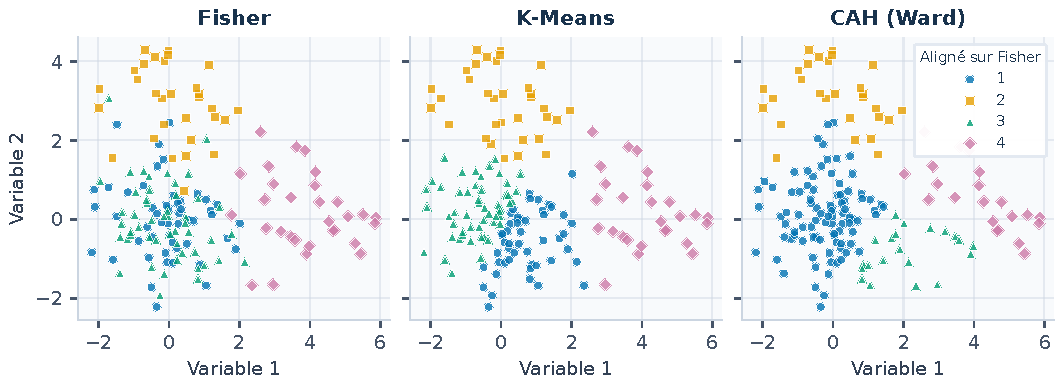
\includegraphics[width=0.98\linewidth,height=4.8cm,keepaspectratio]{simulation_espace.pdf}
\caption[Simulation : partitions dans l'espace]{Partitions dans le plan des deux variables. Les couleurs sont alignées
sur Fisher : les segments 1 et 3 se recouvrent spatialement.}
\label{fig:simuespace}
\end{figure}

\begin{figure}[H]
\centering
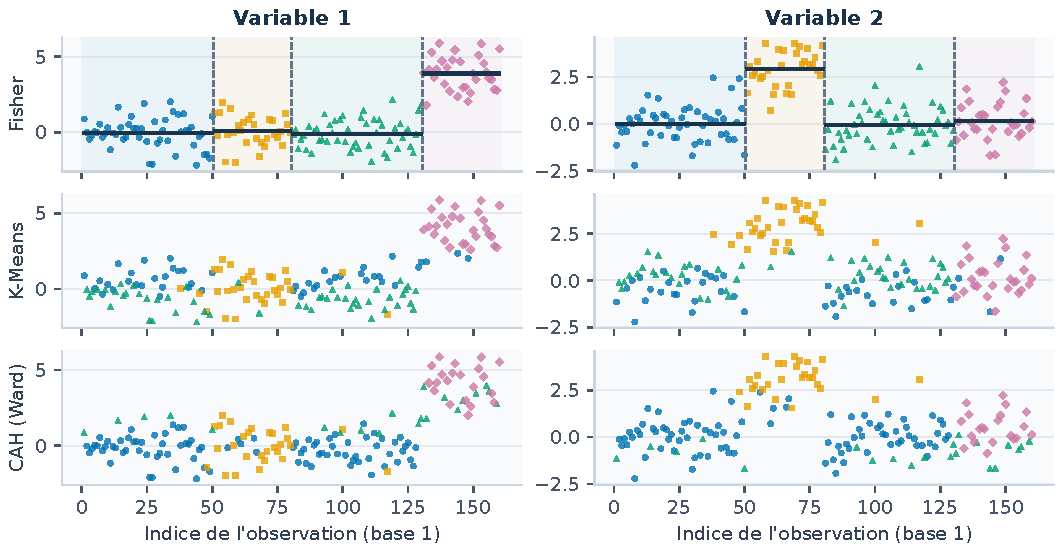
\includegraphics[width=0.98\linewidth,height=7.4cm,keepaspectratio]{simulation_temps.pdf}
\caption[Simulation : partitions selon l'ordre des observations]{Partitions à $K=4$ selon l'ordre des observations ; pointillés :
coupures Fisher ; traits horizontaux : moyennes ajustées par segment.
Les couleurs sont alignées sur les segments Fisher.}
\label{fig:simutemps}
\end{figure}
\begin{table}[H]
\centering\small
\begin{tabular}{lrr}
\toprule
Méthode & Inertie & Changements voisins \\
\midrule
Fisher & 300{,}60 & 3 \\
K-Means & 202{,}89 & 75 \\
CAH (Ward) & 246{,}58 & 45 \\
\bottomrule
\end{tabular}

\caption[Simulation : inertie et changements de label]{Inertie et nombre de changements de label entre observations voisines.}
\label{tab:simucomparaison}
\end{table}

Le recouvrement des segments 1 et 3 (figure~\ref{fig:simuespace}) explique
que les méthodes non contraintes regroupent des points de périodes différentes.
Leur inertie plus faible traduit une meilleure compacité spatiale, mais les
alternances de labels révèlent une fragmentation temporelle. Fisher préserve
la cohérence des régimes successifs. Sans étiquettes de référence, cette
comparaison ne mesure toutefois pas l'exactitude des partitions.

\section{Application aux données réelles : aiguillage}
L'analyse porte sur quatre classes. Les transitions de la colonne 553 donnent
les coupures Python $[35,75,120]$ ; en numérotation à partir de 1, les débuts
des nouveaux segments sont $[36,76,121]$. Fisher retrouve exactement ces limites
et les effectifs $[35,40,45,20]$.

\begin{figure}[H]
\centering
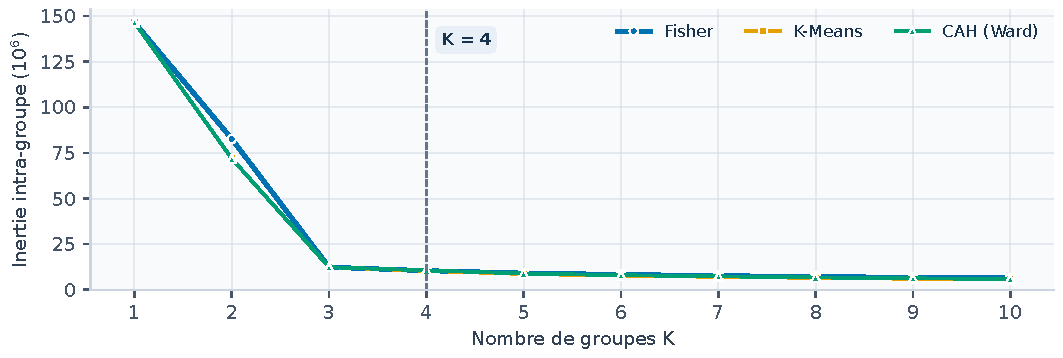
\includegraphics[width=0.94\linewidth,height=4.5cm,keepaspectratio]{aiguillage_coude.pdf}
\caption[Aiguillage : inerties selon le nombre de classes]{Inerties sur \file{aiguillage}. Le trait vertical indique $K=4$,
fixé pour la comparaison avec les quatre classes de référence.}
\label{fig:reelcourbes}
\end{figure}
La décroissance ralentit nettement après $K=3$
(figure~\ref{fig:reelcourbes}). Les quatre classes sont ici connues :
$K=4$ sert à évaluer leur reconstitution, indépendamment de ce coude.

\begin{table}[H]
\centering\small
\begin{tabular}{lrrrr}
\toprule
Méthode & ARI & Corrects & TBC & Changements \\
\midrule
Fisher & 1{,}000 & 140/140 & 100{,}00\,\% & 3 \\
K-Means & 0{,}943 & 137/140 & 97{,}86\,\% & 9 \\
CAH (Ward) & 0{,}859 & 132/140 & 94{,}29\,\% & 7 \\
\bottomrule
\end{tabular}

\caption[Aiguillage : ARI, TBC et changements de label]{Résultats sur les 140 observations, dans l'espace brut à 552 variables.
Le TBC suit l'alignement optimal ; K-means utilise 20 départs, graine 42.}
\label{tab:reel}
\end{table}

\begin{figure}[H]
\centering
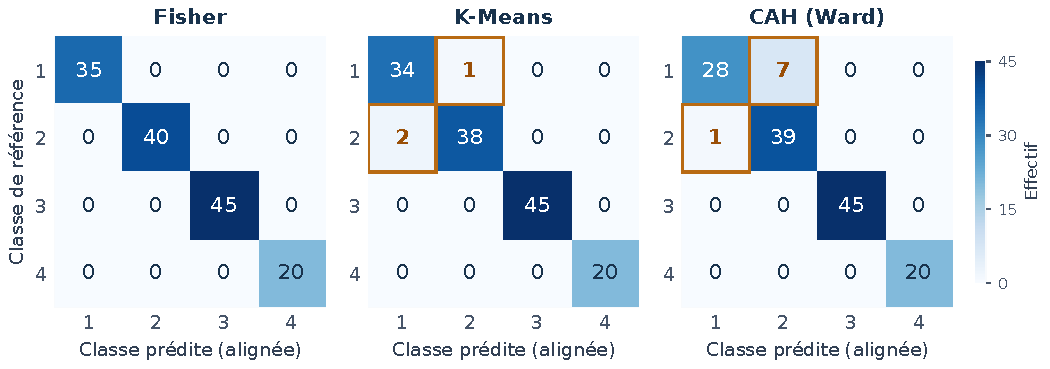
\includegraphics[width=0.98\linewidth,height=5.5cm,keepaspectratio]{aiguillage_confusion.pdf}
\caption[Aiguillage : matrices de confusion]{Matrices de confusion après permutation optimale des labels.
Les lignes sont les classes de référence ; les colonnes, les classes prédites.
L'échelle de couleur est commune ; les cellules encadrées signalent les erreurs.}
\label{fig:confusion}
\end{figure}

Les erreurs se lisent directement dans la figure~\ref{fig:confusion}.
Fisher classe les 140 observations conformément à la référence.
Les K-means affectent une observation de la classe 1 à la classe 2 et deux
dans le sens inverse : 137 observations sont correctement affectées.
Ward confond sept observations de la classe 1 avec la classe 2 et une dans
le sens inverse, soit 132 bonnes affectations. Les classes 3 et 4 sont
intégralement retrouvées par les trois méthodes.

\begin{figure}[H]
\centering
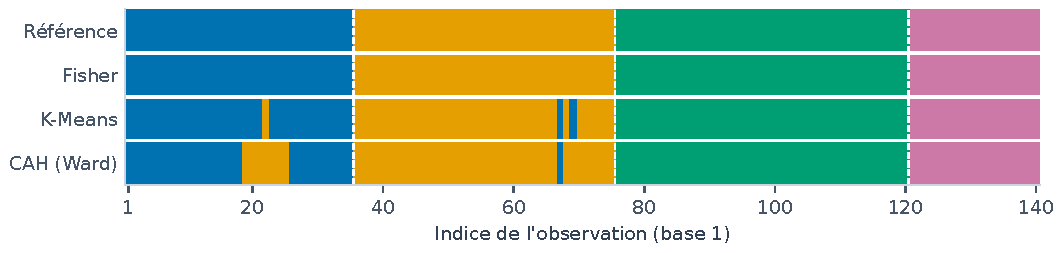
\includegraphics[width=0.98\linewidth,height=3.2cm,keepaspectratio]{aiguillage_ordre.pdf}
\caption[Aiguillage : labels selon l'ordre d'acquisition]{Labels selon l'ordre d'acquisition. Une même couleur représente la
même classe alignée dans les quatre lignes ; les pointillés séparent les
segments retrouvés par Fisher.}
\label{fig:ordre}
\end{figure}

La figure~\ref{fig:ordre} montre que les erreurs des comparateurs introduisent
des allers-retours entre les deux premiers régimes. Les K-means ont un meilleur
TBC que Ward, mais davantage de changements de label (9 contre 7) : l'accord
à la référence et la continuité temporelle ne sont donc pas équivalents.

\begin{figure}[H]
\centering
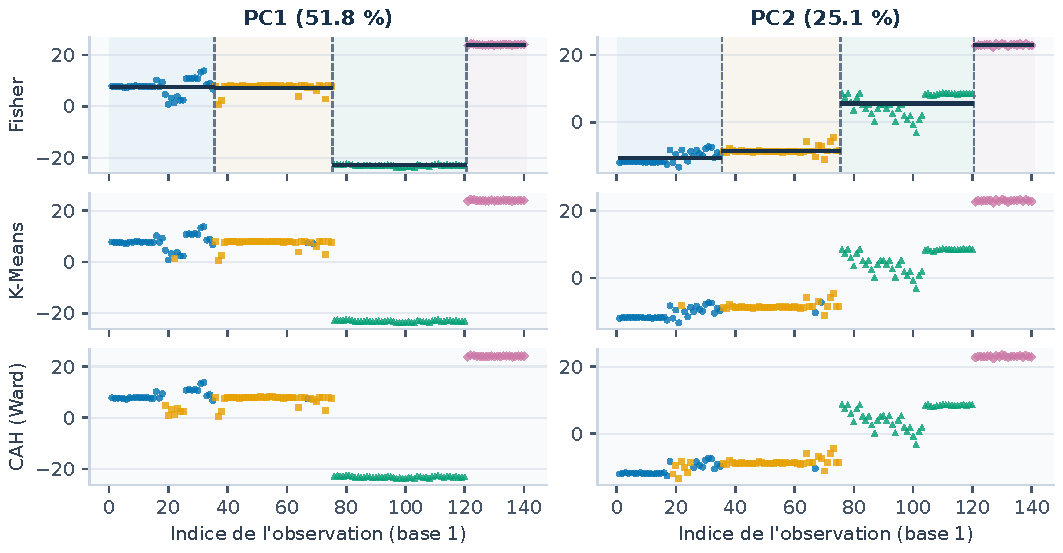
\includegraphics[width=0.98\linewidth,height=7.4cm,keepaspectratio]{aiguillage_temps.pdf}
\caption[Aiguillage : composantes principales selon l'ordre]{PC1 et PC2 selon l'indice d'observation. Les pointillés délimitent les
segments Fisher ; les traits horizontaux indiquent leurs moyennes projetées.
Les couleurs sont alignées sur la référence. L'ACP centrée-réduite sert à
l'affichage ; les partitions sont ajustées sur les 552 variables brutes.}
\label{fig:reeltemps}
\end{figure}
Les moyennes par segment dans la figure~\ref{fig:reeltemps} rendent visibles
les régimes successifs dans cette projection.

La décomposition de Huygens $I=I_W+I_B$ \cite{same} est vérifiée
numériquement. L'inertie et l'accord à la référence restent deux critères distincts :
les K-means ont une inertie de $10{,}346\times10^6$, contre
$10{,}458\times10^6$ pour Fisher et $10{,}599\times10^6$ pour Ward,
sans retrouver tous les labels.
Les K-means peuvent réduire la dispersion en regroupant des observations non
contiguës ; l'inertie seule ne mesure donc pas l'accord à la référence.

\section{Sensibilité et interprétation}
\label{sec:sensibilite}
Les analyses suivantes évaluent la sensibilité des résultats au nombre
d'initialisations, à la graine aléatoire et à la standardisation.

\subsection{Initialisation des K-means et choix d'échelle}
À graine 42 et $K=4$ constants, le TBC passe de $63{,}57\,\%$ à
$97{,}86\,\%$ entre un et 20 départs (tableau~\ref{tab:restarts}).
Aucun gain supplémentaire n'est observé entre 10, 20 et 50 départs pour cette
graine. Avec 20 départs, les graines 0 à 9 donnent encore des ARI de
$0{,}925$ à $0{,}943$ : les répétitions ne garantissent donc pas l'optimum global.

\begin{table}[H]
\centering\small
\begin{tabular}{rrrr}
\toprule
\texttt{n\_init} & ARI & TBC & Inertie ($10^6$) \\
\midrule
1 & 0{,}558 & 63{,}57\,\% & 10{,}6906 \\
10 & 0{,}943 & 97{,}86\,\% & 10{,}3462 \\
20 & 0{,}943 & 97{,}86\,\% & 10{,}3462 \\
50 & 0{,}943 & 97{,}86\,\% & 10{,}3462 \\
\bottomrule
\end{tabular}

\caption[K-means : sensibilité au nombre de départs]{Effet du nombre de départs, données réelles brutes, graine 42.}
\label{tab:restarts}
\end{table}

La standardisation ramène chaque variable à une variance unitaire
\cite{same} et change ainsi la métrique de segmentation.
Appliquée aux trois méthodes avant ajustement, elle dégrade ici leur ARI
(tableau~\ref{tab:scaling}). La première coupure Fisher passe de 35 à 21
en indices Python. Nous conservons les données brutes pour l'expérience
principale. Le déplacement de la frontière montre que les régimes détectés
dépendent de la pondération des coordonnées. Les inerties obtenues sur des
échelles différentes ne sont pas directement comparables.

\begin{table}[H]
\centering\small
\begin{tabular}{lrrr}
\toprule
Données & Fisher & K-Means (20 départs) & Ward \\
\midrule
Brutes & 1{,}000 & 0{,}943 & 0{,}859 \\
Standardisées & 0{,}781 & 0{,}735 & 0{,}545 \\
\bottomrule
\end{tabular}

\caption[ARI : sensibilité à la standardisation]{ARI à $K=4$ selon le prétraitement ; K-means à 20 départs, graine 42.}
\label{tab:scaling}
\end{table}

\begin{figure}[H]
\centering
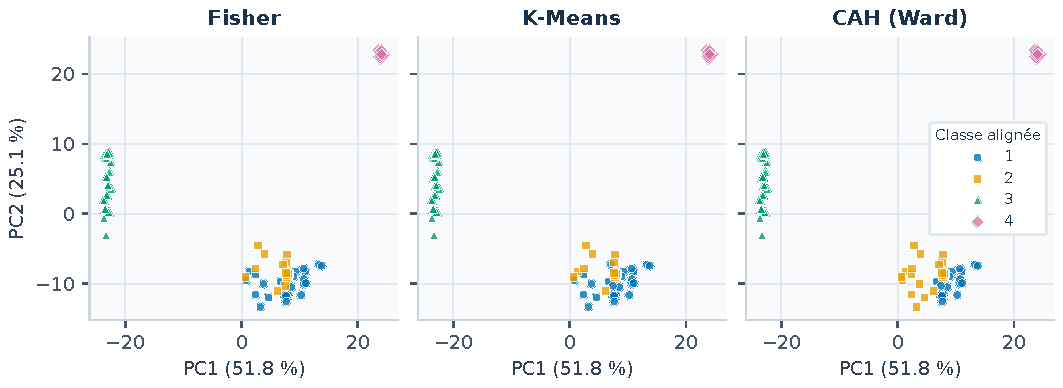
\includegraphics[width=0.98\linewidth,height=4.8cm,keepaspectratio]{aiguillage_espace.pdf}
\caption[Aiguillage : projection ACP des partitions]{Projection ACP des données centrées-réduites, colorée par les partitions
ajustées sur les variables brutes. PC1 et PC2 expliquent respectivement
\PcaOne\,\% et \PcaTwo\,\% de la variance ; les couleurs sont alignées sur la référence.}
\label{fig:acp}
\end{figure}

Dans la projection ACP (figure~\ref{fig:acp}), les classes 1 et 2 se recouvrent
davantage que les classes 3 et 4, ce qui est cohérent avec la localisation des
erreurs. Cette lecture reste partielle : environ $77\,\%$ de la variance
standardisée est représentée. Les 140 observations comprennent 128 vecteurs
distincts ; les répétitions, toutes dans la classe 3, sont conservées pour
respecter l'ordre d'acquisition.

\section{Conclusion}
Fisher distingue des régimes successifs proches dans l'espace.
La contrainte d'ordre permet ici de retrouver exactement
la partition de référence de \file{aiguillage}, tandis que les comparateurs
introduisent quelques affectations isolées entre les deux premiers régimes.
Les départs multiples des K-means réduisent nettement l'écart, et la
standardisation modifie les frontières. La pertinence de la segmentation dépend
donc à la fois de l'ordre des observations et de la métrique retenue.

\clearpage
\begingroup
\titleformat{name=\section,numberless}{\centering\large\bfseries\color{navy}}{}{0pt}{}
\phantomsection
\addcontentsline{toc}{section}{Références}
\small
\setlength{\parskip}{0pt}
\begin{thebibliography}{6}
\setlength{\itemsep}{0.3em}
\bibitem{fisher}
W. D. Fisher (1958).
On Grouping for Maximum Homogeneity.
\emph{Journal of the American Statistical Association}, 53(284), 789--798.
\href{https://doi.org/10.1080/01621459.1958.10501479}{doi:\,\nolinkurl{10.1080/01621459.1958.10501479}}.

\bibitem{lloyd}
S. P. Lloyd (1982).
Least Squares Quantization in PCM.
\emph{IEEE Transactions on Information Theory}, 28(2), 129--137.
\href{https://doi.org/10.1109/TIT.1982.1056489}{doi:\,\nolinkurl{10.1109/TIT.1982.1056489}}.

\bibitem{ward}
J. H. Ward, Jr. (1963).
Hierarchical Grouping to Optimize an Objective Function.
\emph{Journal of the American Statistical Association}, 58(301), 236--244.
\href{https://doi.org/10.1080/01621459.1963.10500845}{doi:\,\nolinkurl{10.1080/01621459.1963.10500845}}.

\bibitem{sklearn}
Scikit-learn 1.8.0.
\emph{KMeans : paramètres init et n\_init}.
Documentation officielle, consultée le 21 novembre 2026.
\url{https://scikit-learn.org/1.8/modules/generated/sklearn.cluster.KMeans.html}.

\bibitem{hubert}
L. Hubert et P. Arabie (1985).
Comparing Partitions.
\emph{Journal of Classification}, 2, 193--218.
\href{https://doi.org/10.1007/BF01908075}{doi:\,\nolinkurl{10.1007/BF01908075}}.

\bibitem{same}
A. Samé (s. d.).
\emph{Clustering — Master MLSD}.
Université Gustave Eiffel, supports de cours officiels :
\emph{Introduction} (chap.~1, p.~31 et pp.~53--67) ;
\emph{Classification hiérarchique} (chap.~2, pp.~36--39) ;
\emph{Méthodes par partitionnement} (chap.~3, pp.~4--13, 47--49 et 61--64).
Pagination des fichiers PDF.
\end{thebibliography}
\endgroup

\end{document}
